%! Author = mumoe
%! Date = 4/13/2022

% Preamble
\documentclass[../main.tex]{subfiles}

\begin{document}

\onehalfspacing

En este capítulo, se mostrarán los resultados obtenidos en este trabajo. Se da un enfoque para cada una de las redes mostradas en el capítulo de metodología.%Y finalizando en incorporar las dos ideas para incorporar

Por un lado, el análisis de cada una de las $NC(h)$ se realizó a través del cálculo de métricas mostradas en el apartado de marco teórico.  Por otro lado, en la red de prexplosividad $\G{h}$, se realizó un análisis en las comunidades obtenidas y cómo estas pueden favorecer el comportamiento explosivo a través del uso de las mismas métricas antes mencionadas.

Se analizaron 150 tendencias al realizar una limpieza a la base datos. El filtro se basó en considerar aquellas tendencias que tienen más de 4000 tweets. El etiquetado de su comportamiento fue hecho de manera manual al analizar su respectiva serie de tiempo (ver figura \ref{fig:introducction_timeserie_example} como ejemplo ).
%De forma específica, por cada periodo de tiempo $t$ se usaron métricas locales y globales (véase la sección de marco teórico) en $NC_{t}^{T}(h)$ y $NC_{t}^{R}(h)$.


\section{Análisis de comunidades.}

En esta sección, se analizará con detalle dos momentos importantes en la dinámica de las tendencias: Minutos previos a la mayor interacción y el momento de la mayor interacción.  Se usó el tiempo $t^{*}$ donde es la hora donde se recapituló la mayor interacción en la red $NC_{t^{*}}(h)$ y la red $\G{h}$ sobre los periodos de 25 a 50 minutos antes del periodo $t^{*}$ como se mencionó con más detalle en la sección de metodología.


\subsection{Comunidades comprometidas y homogéneas.}

Cabe recordar que la principal diferencia entre las redes $\G{h}$ y $NC^{T}_{t^{*}}(h)$ es la escala y tiempo de análisis. Por lo que, al analizar la red $NC^{T}_{t^{*}}(h)$ estamos interesados a la dinámica completa del comportamiento explosivo en el momento del pico de interacci
ón. Por otro lado, de la red $\G{h}$ nos interesa conocer más sobre la estructura de la red social que llevó al comportamiento antes mencionado. Considerar esta distinción permite diferenciar los resultados desde una perspectiva cualitativa y otra desde un enfoque predictivo.



En el primer caso, obtendremos el grado de asortatividad $(r)$de la red $NC_{t^{*}}^{T}(h)$. Esa métrica es para denotar distribuciones de grado heterogéneas. La diferencia entre entre ellas resulta ser significativa (95\% de confianza ).  El valor $r$ puede denotar con la existencia de usuarios \textit{puente} cuando $r$ sea negativo. De la figura \ref{fig:results_RmaxInteract}, notemos el sesgo de los valores de $r$ en la tendencias de comportamiento explosivo. Del mismo gráfico, podemos denotar que la estructura de la red, debe ser levemente disortativa; lo cual, nos resalta la necesidad de estos nodos o usuarios puente.


\begin{figure}
    \centering
    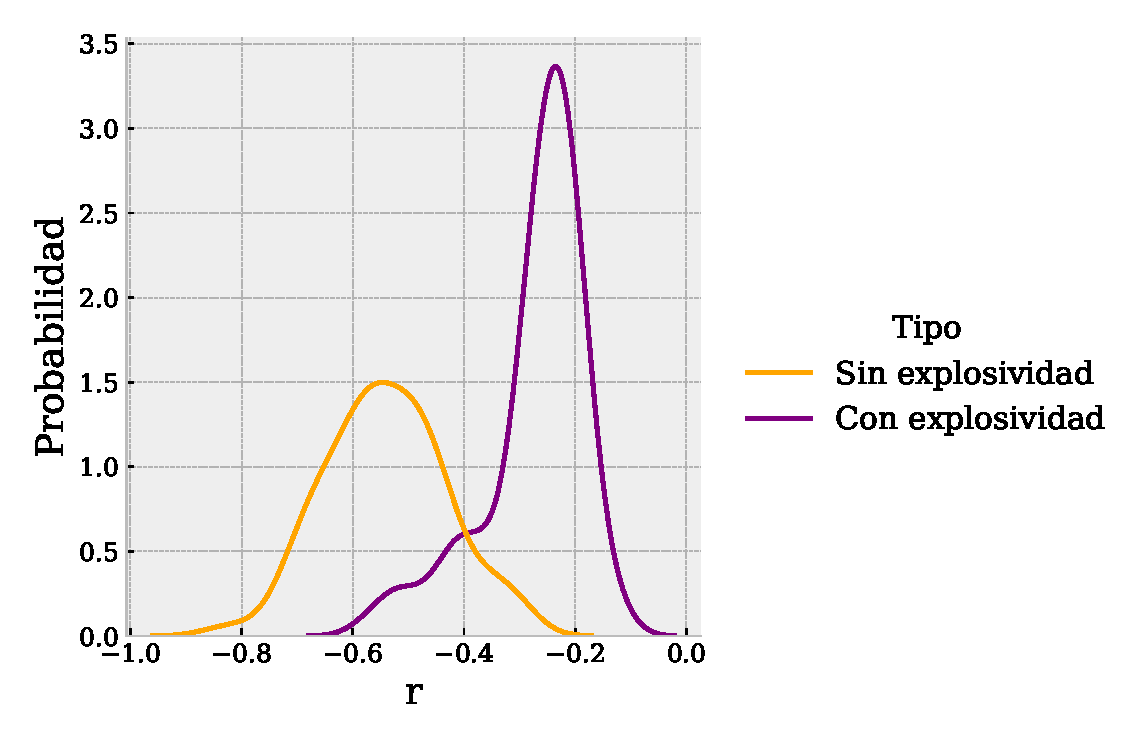
\includegraphics[scale = 0.7]{images/results_Rmaxinteract.pdf}
    \caption{Histograma de la asortatividad de las redes por su tipo de comportamiento. La diferencia en medias es significativa.  }
    \label{fig:results_RmaxInteract}
\end{figure}
% \myfigure{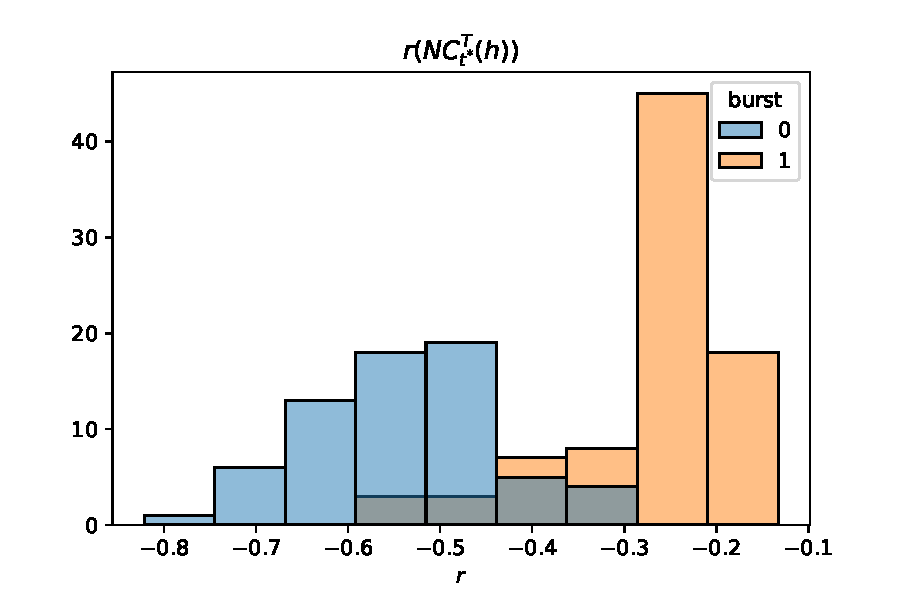
\includegraphics[width=.9\columnwidth]{images/hist_r_max.pdf}%
% \figcaption{Histograma del valor $r$ por su tipo de comportamiento. Notemos como existe un sesgo significativo que caracterizan a las tendencias.}}

Por otro lado, los datos obtenidos de las redes $\G{h}$ complementan esta nueva versión. De la figura \ref{fig:resultados_lenComunidades} , podemos ver cómo las tendencias con comportamiento explosivo deben tener un mayor número de comunidades interactuando; la diferencias son denotadas por el cadro \ref{tab:resulatdos_comparativodecomunidades}.

\begin{table}[]
    \centering
    \caption{Comparativo de las estadísticas de la cantidad de comunidades antes de la mayor interacción.}
    \label{tab:resulatdos_comparativodecomunidades}
    \begin{tabular}{lrr}
\toprule
{} &  Explosividad &  Sin explosividad \\
\midrule
Media  &    167.951807 &         99.416667 \\
$\sigma$   &     78.834019 &         85.424422 \\
min   &      8.000000 &          6.000000 \\
25\%   &    124.000000 &         40.750000 \\
50\%   &    175.000000 &         66.500000 \\
75\%   &    208.000000 &        125.500000 \\
max   &    363.000000 &        418.000000 \\
\bottomrule
\end{tabular}
\end{table}


Además, es clave el factor tiempo entre cada interacción y la repetición o insistencia del usuario. La figura \ref{fig:resultados_1000Tweets}  nos da una muestra bastante clara sobre un umbral de interacción repetida; es decir que un mismo usuario repita interacciones. Esta gráfica muestra los usuarios en los primeros mil \textit{tweets} ordenados antes del periodo $t^{*}$ para cada tendencia; siendo $n =1$ el \textit{tweet} más antiguo y $n=1000$ el más reciente. Es la razón de la cantidad de usuarios distintos hasta el $n-esimo$ \textit{tweet}. Formalmente, si ${U_{i} }_{i=1}^{1000}$ es las sucesión de usuarios de los \textit{tweets} antes mencionados, entonces el gráfico de arriba es $\frac{|\cup_{i=1}^{k} U_{i} |}{k}$ para cada $1 \leq k \leq 1000$.
 La interpretación de la misma es sencilla:  valores cercanos a 1 es que en cada \textit{tweet} fue hecho por un usuario distinto; mientras que valores cercanos a 0 son \textit{tweets} hecho por un mismo usuario. El grosor de cada línea es proporcional al tiempo que hay entre cada $tweet$. De este gráfico podemos reconocer la importancia que el tiempo entre las interacciones y el número de interacciones únicas influye en la explosividad de la tendencia.

\begin{figure}
    \centering
    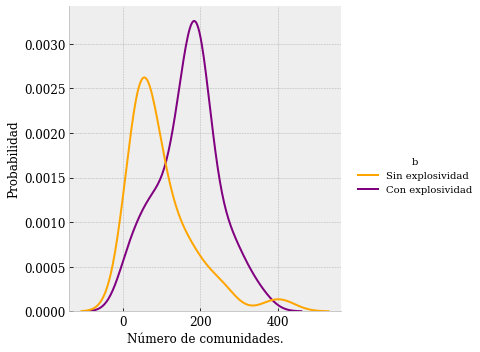
\includegraphics[scale = 0.6]{images/resultados_comparativocomunidades.png}
    \caption{Histograma del número de comunidades de las redes $\G{h}$ por su tipo de comportamiento. Notemos como existe un sesgo significativo que caracterizan a las tendencias.}
    \label{fig:resultados_lenComunidades}
\end{figure}



%\newpage



% Así, a partir de estos nuevos datos sobre las estadísticas de la $\G{h}$ se propone un árbol de decisión que permita, a través de los valores encontrados de los usuarios partícipes en los 50 y 25 minutos antes del comportamiento. De este último algoritmo, se obtiene un score del $0.81$. De este mismo árbol, se nota que los primeros nodos clasificadores está asociados a métricas globales de la red en cuestión. Así mismo, la variable $mean\_nt$ es el número promedio de $tweets$ en cada periodo, también resulta relevantes para la caracterización de las tendencias de comportamiento explosivo misma que se puede concluir del gráfico 11 sobre los tiempos de interacción. Por lo tanto, si bien el árbol clasificador considera métricas de centralidad sobre estos usuarios partícipes, es mucho más relevante la topología de la red en sí.


% \section{Discusión antes del momento del pico de interacción.  }


% \begin{figure}[h!]
%     \centering
%     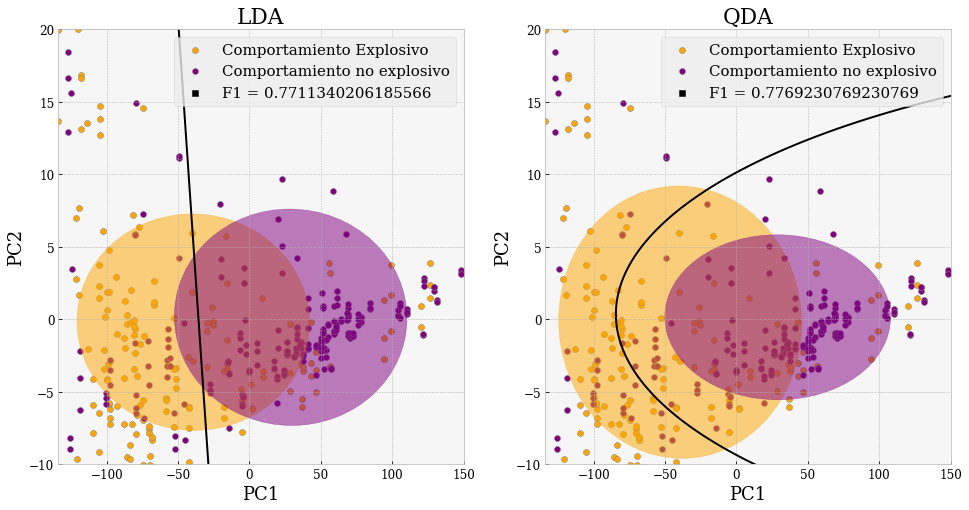
\includegraphics[scale = 0.45]{images/resultados_discriminantes.png}
%     \caption{Caption}
%     \label{fig:my_label}
% \end{figure}


\begin{figure}
    \centering
    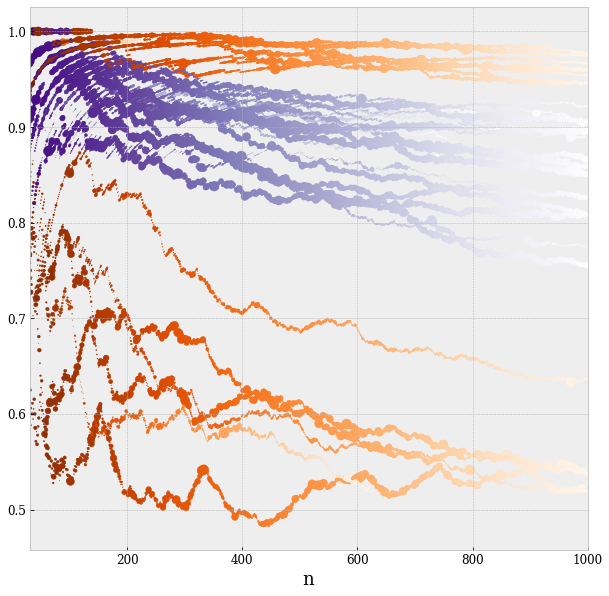
\includegraphics[scale = 0.5]{images/resultados_razonusuarios.png}
    \caption{ Comparativo de tendencias por los primeros 1000 \textit{Tweets}. Razón de usuarios nuevos en cada \textit{tweet} de los 1000 \textit{tweets} antes del periodo $t^{*}$. La líneas de color morado corresponden a tendencias con comportamiento explosivo.  }
    \label{fig:resultados_1000Tweets}
\end{figure}

\section{Análisis global de la dinámica de las tendencias.}


En esta sección, se explicará con detalle el cálculo que se realizó para la red $NC_{t}^{T}(h)$ por cada tendencia $h$. Cabe recordar que la red $NC(h)$ es una red temporal multicapa, por lo cual $NC^{T}(h)$ es una red no dirigida y $NC_{t}^{R}(h)$ es una red dirigida donde $t$ es un periodo de tiempo fijo. Cada uno en estas redes representa a un usuario que participó con algún tweet o retweet en el periodo de tiempo $t$.


%Agregar una tabla donde comparemos métricas simples por tipo de
Se puede notar la diferencia entre la cantidad de usuarios partícipes es diferente de las tendencias con comportamieno explosivo. En las tablas \ref{tab:my_label_0} y \ref{tab:my_label_1}, al tener una mayor cantidad de usuarios es esperable tener una mayor cantidad de tweets, sin embargo el hecho de tener una gran audiencia no es suficiente para caraterizar las tendencias del gráfico \ref{fig:resultados_comparativotweetsusuarios}, no hay diferenciador para las tendencias con comportamiento explosivo.

\begin{figure}
    \centering
    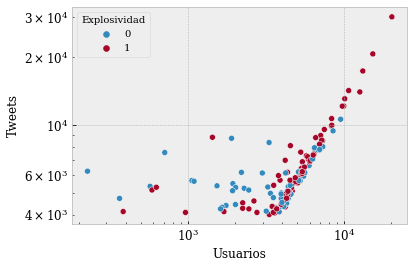
\includegraphics[scale = 0.8]{images/resultados_comparativoTweets.png}
    \caption{Comparativo de tendencias por la cantidad de usuarios registrados respecto a la cantidad de tweet recabados. }
    \label{fig:resultados_comparativotweetsusuarios}
\end{figure}

Con esto en mente, es factible aplicar diversas métricas conocidas de redes. Por ejemplo, para la red $NC_{t}^{T}(h)$ se puede calcular el coeficiente de asortatividad y para $NC_{t}^{R}$ se puede obtener la media del grado exterior.


\begin{table}[!h]
    \centering
    \caption{Comparativo entre las tendencias por el número de usuarios totales que interactuaron en ella. }
    \label{tab:comparativo_tendenciasnumerosdetweets}
    \begin{tabular}{cc}
    \begin{minipage}{.5\linewidth}
        \begin{tabular}{ll}
            \toprule
                 Tendencia &  Usuarios  \\
\midrule
        \textit{wheniwaslittle} &        20150  \\
   \textit{yougetmajorpointsif} &        15219  \\
            \textit{top100lies} &        13129  \\
 \textit{nationalbestfriendday} &        12569  \\
\textit{mythoughtsduringschool} &        10662  \\
\bottomrule
        \end{tabular}
    \end{minipage} &

    \begin{minipage}{.5\linewidth}
        \begin{tabular}{ll}
            \toprule
 Tendencia &  Usuarios  \\
\midrule
   \textit{fml} &         9467 \\
   \textit{wtf} &         8467 \\
  \textit{fail} &         7283 \\
  \textit{2omf} &         6957 \\
\textit{ohwell} &         6915 \\
\bottomrule
        \end{tabular}
    \end{minipage}
\end{tabular}
\end{table}



Con esto en mente, se realizaron los siguientes cálculos, especificando en qué red fue aplicada.

\begin{itemize}
    \item Para cada $NC_{t}^{T}$ donde $t$ es una ventana de tiempo.
    \begin{enumerate}
        \item Grado promedio.
        \item Media del camino más corto.
        \item Cálculo de la métrica clustering
        \item Cálculo de la métrica betweenness %Esta no pasa KruskalWallis
        \item Cálculo de la entropía de Shannon de la distribución de grado.
        \item Grado promedio
    \end{enumerate}
    \item Para cada $NC_{t}^{R}$
    \begin{enumerate}
        \item Grado exterior más grande.
        \item Diámetro más grande.
    \end{enumerate}
\end{itemize}

De cada tendencia se obtuvo una serie de tiempo por cada una de las métricas. Para inferir un valor característico en cada una de estas métricas, se procedió a calcular un estadístico en cada una de estas serie de tiempo. Por un lado, para las métricas relacionadas a la red no dirigida $(NC_{t}^{T})$ se procedió a obtener la media de cada una de las  series de tiempo. Por otro lado, para las red dirigida, se procedió a calcular el máximo valor de esta serie de tiempo.

A partir del cálculo de estos estadísticos, se empiezan a notar diferencias entre las tendencias. Se puede notar de la tabla \ref{tab:resultados_diferenciasDeTendencias} que la diferencia entre el comportamiento de tendencias resulta ser estadísticamente significativo a través de la prueba de Kruskal-Wallis %(95\% de confianza) (ver pruebas paramétricas en anexo X).
% También puede ser (en el anexo X se puede consultar las pruebas paramétricas)

\begin{table}[h!]
    \centering
    \caption{Valores $p$ obtenidos al aplicar la prueba no paramétrica de Kruskal-Wallis. }
    \begin{tabular}{lr}
\toprule
      Estadística  &       \textit{Valor $P$} \\
\midrule
     Media de la cantidad de Tweets por hora  &  $1.585502\text{x}10^{-16}$ \\
   Media de la cantidad de retweets &  $2.797278\text{x}10^{-18} $\\
    Media del grado promedio &  \textbf{$5.785002\text{x}10^{-02}$} \\
    Media del promedio de longitud del camino más corto   &  $2.423004\text{x}10^{-20}$ \\
  Media del clustering &  $1.419858\text{x}10^{-07}$ \\
 Media del betweenness &  \textbf{$2.560294\text{x}10^{-01}$} \\
     Media de la entropía &  $2.288698\text{x} 10^{-18}$ \\
     Diámetro más grande &  $4.843335\text{x} 10^{-14}$ \\
        Vecindad más grande &  $1.283606\text{x} 10^{-15}$ \\
\bottomrule
\end{tabular}
    \label{tab:resultados_diferenciasDeTendencias}
\end{table}


% \section{ Valores significativos en la entropía, clustering y betweenness. }
\subsection{ Valores significativos en la dinámica total y en el pico de interacción.  }




% La distribución de grado de una red provee un primer acercamiento a la investigación de la red en cuestión. Al considerar la distribución de grado como una probabilidad, permite el uso de diversas herramientas probabilísticas como la  entropía de Shannon. El estudio de esta métrica aplicada en redes ha sido corto y en casos muy particulares: En el caso de redes de acitvida neuronal, la entropía de Shannon fue útil para no descartar la teoría entrópica del cerebro  \cite{ayahuasca_Viol2017} o, en un hiperplano meramente matemático, se concluyó que la entropía de la distribución de grado es una medida efectiva de la resiliencia de la red en ataques aleatorios \cite{entropia_opti}. En ambos artículos, se destaca un uso de la entropía de Shannon en la distribución de grado para destacar a la red diferencias no obvias de redes.
Con esto último en mente, se procede al desarrollo y análisis de los resultados.

\begin{figure}[h!]
    \centering
    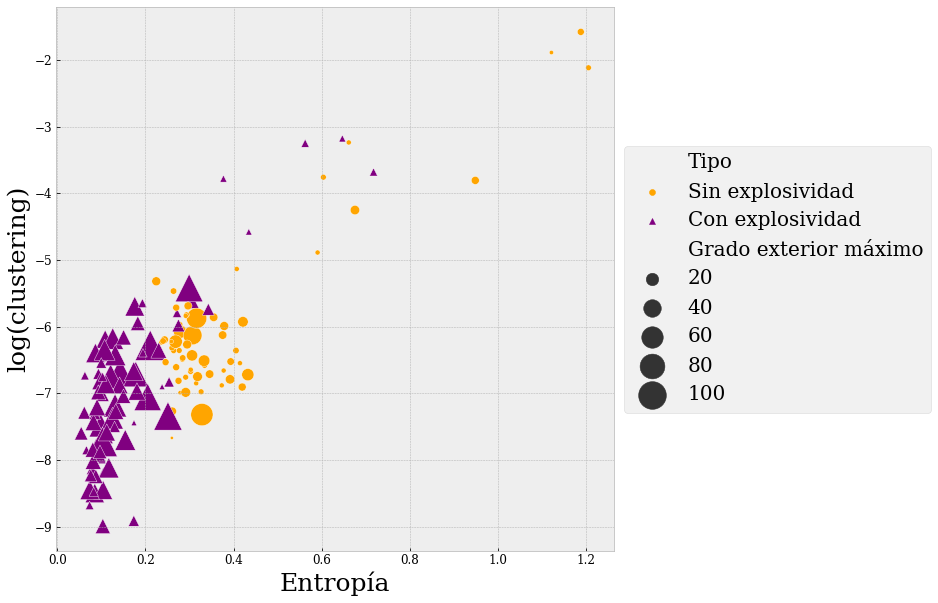
\includegraphics[scale = 0.40]{images/results_entropyVSclustering.png}
    \caption{Comparativo entre las tendencias respecto a las métricas calculadas. El tamaño de cada uno de los marcadores es proporcional al máximo del grado exterior máximo de cada una de las tendencias. }
    \label{fig:results_entropyVSclustering}
\end{figure}

La entropía de Shannon ( ver \ref{shannon-entropy}) es una medida de incertidumbre para una variable aleatoria. Por su propia construcción, es positiva  y  no se enfoca en los valores de la variable aleatoria; se da énfasis en la probabilidad de los eventos mas no el evento en sí. Se especifica en la incertidumbre del estado actual.


En las figura \ref{fig:results_entropyVSclustering} y \ref{fig:results_entropyVSbetweeness}, podemos ver las relaciones entre el comportamiento explosivo y el valor de su entropía contra otras métricas. Si bien, tenemos datos atípicos, la tendencias con comportamiento no explosivo tuvieron un valor mínimo en su entropía (0.25 aprox.). En consecuencia de la misma interpretación de la entropía de Shannon, esto nos induce a que la red de las tendencias con comportamiento explosivo son homogéneas en su distribución de grado.

\begin{figure}[h!]
    \centering
    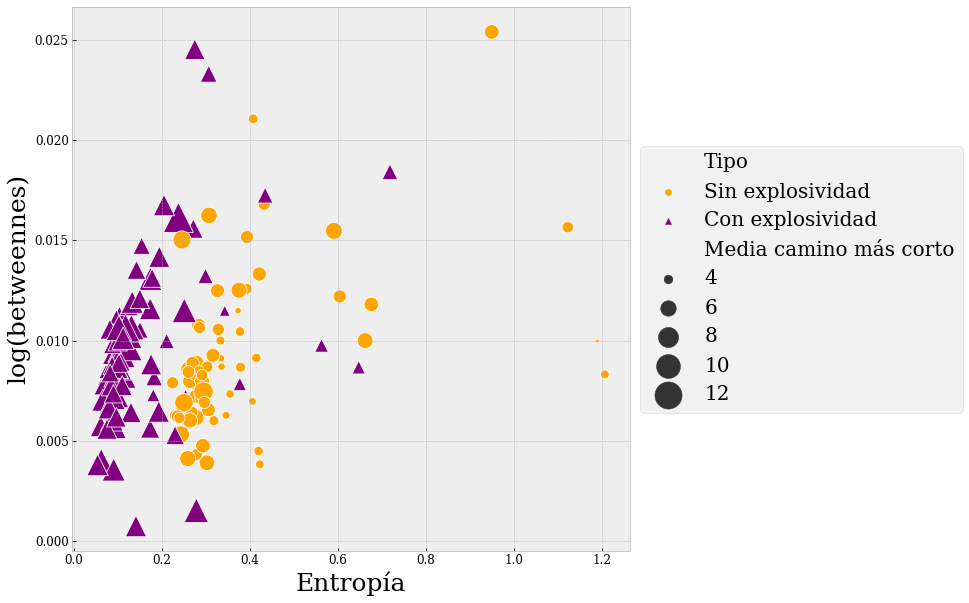
\includegraphics[scale = 0.40]{images/results_entropyVSbetweennes.png}
    \caption{Comparativo de tendencias a través de la media de las métricas betweenness y entropia. El tamaño de cada uno de los marcadores del gráfico está en proporción de la media del camino más corto. }
    \label{fig:results_entropyVSbetweeness}
\end{figure}

De la misma manera, este análisis mostró relaciones interesantes entre las métricas betweenness y la entropía. Del gráfico \ref{fig:results_entropyVSclustering}, podemos ver una clara correlación lineal positiva entre la entropía y la métrica clustering. Una correlación esperable ya que al incrementar el clustering,se incrementa el número triángulos y, por tanto, un cambio en el grado de los nodos. Además, siguiendo del mismo gráfico, se puede apreciar como el beneficio de actividades de costo mínimo como los retweets propician que la tendencia sea de comportamiento explosivo.

Esto último puede ser consecuencia del tipo de \textit{tendencia} o tema que se requiera discutir; del artículo \cite{REDDIT} nos dan un pequeño análisis de comunidades sobre \textit{subreddits} (comunidades más pequeñas) mostrando que aquellas con pocas personas pero con una organización clave entre las demás, pueden generar enfrentamientos masivos; misma idea fue hecha \cite{Conover_Ratkiewicz_Francisco_Goncalves_Menczer_Flammini_2011}, sobre discusiones políticas en \textit{Twitter}. Lo cual, al considerar la poca incertidumbre de la entropía de Shannon, es consistente con la bibliografía de comunidades pequeñas pero organizadas.

Para concluir, se necesita cierta homogeneidad entre comunidades para generar el comportamiento explosivo. Específicamente, que esa homogeneidad no rebase una entropía de 0.25. Por otro lado, notemos que también debe existir la necesidad de acciones de menor costo y con tiempos específicos. La dinámica de \textit{Twitter} es una comunicación sencilla y simple. La acción de \textit{retweet} es la de menor costo y, por tanto, la que recapitula la mayor cantidad de interacción.

\end{document}